\documentclass{beamer}
% Required packages
\usepackage{amsmath}
\usepackage{physics}
\usepackage{graphicx}
\usepackage{siunitx}
\usepackage{xcolor}
\usepackage{tikz}
% Set image search paths
\graphicspath{{../images/}{../../shared/images/}}

% Define custom colors for DS9 theme
\definecolor{ds9blue}{RGB}{25,25,112}
\definecolor{ds9gold}{RGB}{218,165,32}
\definecolor{ds9grey}{RGB}{105,105,105}
\definecolor{ds9red}{RGB}{178,34,34}
% Set up the Madrid theme with custom colors
\usetheme{Madrid}
\usecolortheme{whale}
\setbeamercolor{palette primary}{bg=ds9blue,fg=white}
\setbeamercolor{palette secondary}{bg=ds9grey,fg=white}
\setbeamercolor{palette tertiary}{bg=ds9gold,fg=black}
\setbeamercolor{palette quaternary}{bg=ds9red,fg=white}
\setbeamercolor{structure}{fg=ds9blue}
\setbeamercolor{title}{fg=ds9gold}
\setbeamercolor{subtitle}{fg=ds9gold}
\setbeamercolor{frametitle}{bg=ds9blue,fg=white}
\setbeamercolor{block title}{bg=ds9blue,fg=white}
\setbeamercolor{block body}{bg=ds9grey!20,fg=black}

% Title page information
\title[Power \& Energy Systems]{PHYS11 CH7: Power, Energy \& Human Systems}
\subtitle{Sections 7.7-7.9: Power, Human Energy, and World Energy Use}
\author[Mr. Gullo]{Mr. Gullo}
\date[Fall 2024]{Fall Semester 2024}

\begin{document}

\frame{\titlepage}

% Learning Objectives
\begin{frame}
\frametitle{Learning Objectives}
\begin{block}{After this lesson, you will be able to:}
\begin{itemize}
\item Calculate power by analyzing changes in energy over time
\item Explain human body energy consumption at rest vs. during activity
\item Calculate the conversion of chemical energy in food to useful work
\item Describe the distinction between renewable and nonrenewable energy sources
\item Explain why energy conservation is necessary despite total energy being conserved
\end{itemize}
\end{block}
\end{frame}

% Power Concepts
\begin{frame}
\frametitle{Power: Rate of Energy Transfer}
\begin{block}{Definition}
Power ($P$) is the rate at which work is done or energy is transferred:
\[ P = \frac{W}{t} = \frac{\Delta E}{\Delta t} \]
SI unit: Watt (W) = 1 Joule/second
\end{block}
\begin{block}{Key Equations}
\begin{itemize}
\item Average Power: $P_{avg} = \frac{\Delta E}{\Delta t}$
\item Instantaneous Power: $P = \frac{dE}{dt}$
\item Relation to Force: $P = \vec{F} \cdot \vec{v}$
\end{itemize}
\end{block}
\end{frame}

% Human Energy System
\begin{frame}
\frametitle{Human Energy Systems}
\begin{figure}
    \centering
    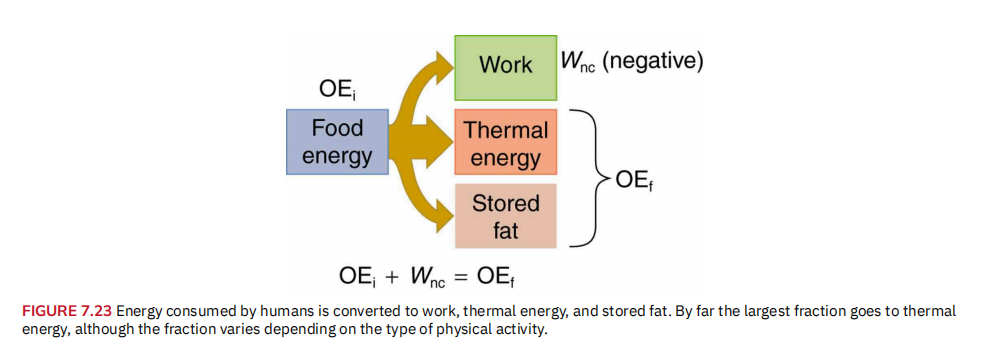
\includegraphics[width=1\linewidth]{CH7/CH7.7-7.9/Screenshot 2024-11-28 120054.png}
\end{figure}
\end{frame}
% Human Energy System
\begin{frame}
\frametitle{Human Energy Systems}
\begin{columns}
\column{0.5\textwidth}
\begin{block}{Basal Metabolic Rate (BMR)}
\begin{itemize}
\item Energy used at rest
\item Typical adult: 70-100 W
\item Major users:
  \begin{itemize}
  \item Liver \& Spleen (27\%)
  \item Brain (19\%)
  \item Muscles (18\%)
  \end{itemize}
\end{itemize}
\end{block}

\column{0.5\textwidth}
\begin{block}{Active Power Output}
\begin{itemize}
\item Walking: 280 W
\item Cycling: 400 W
\item Sprinting: 2415 W
\item Efficiency: 15-30\%
\end{itemize}
\end{block}
\end{columns}
\end{frame}

% World Energy Use
\begin{frame}
\frametitle{World Energy Use}
\begin{figure}
    \centering
    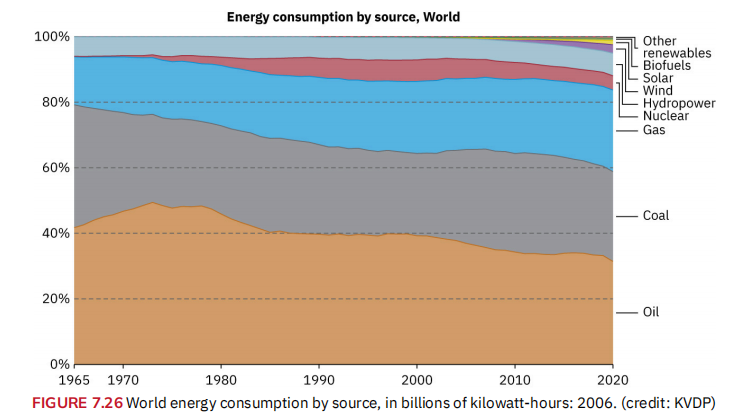
\includegraphics[width=0.9\linewidth]{CH7/CH7.7-7.9/Screenshot 2024-11-28 120155.png}
\end{figure}
\end{frame}

% World Energy Use
\begin{frame}
\frametitle{World Energy Use}
\begin{figure}
    \centering
    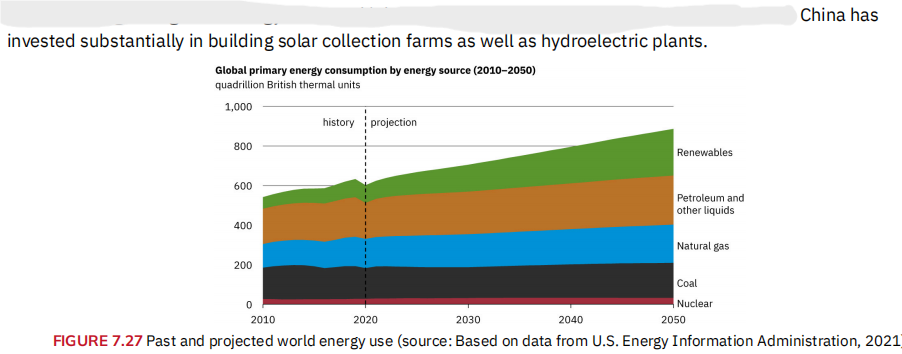
\includegraphics[width=1\linewidth]{CH7/CH7.7-7.9/Screenshot 2024-11-28 1202152.png}
\end{figure}

\end{frame}
\begin{frame}
\frametitle{World Energy Use}
\begin{figure}
    \centering
    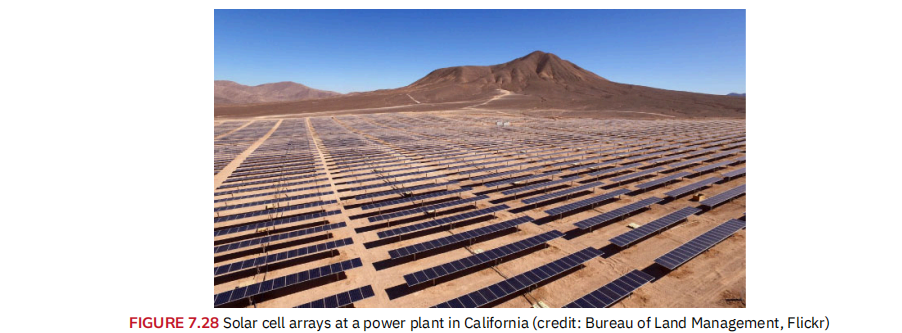
\includegraphics[width=1\linewidth]{CH7/CH7.7-7.9/Screenshot 2024-11-28 120215.png}
\end{figure}

\end{frame}
% Example Problem - I Do
\begin{frame}
\frametitle{Example: Calculating Power Output}
\begin{block}{Problem}
A 60.0-kg person climbs stairs at a rate of 116 stairs per minute. If each stair is 0.15 m high, what is their power output?
\end{block}

\pause

\begin{block}{Solution}
\begin{align*}
\text{Work per stair} &= mgh = (60.0\text{ kg})(9.80\text{ m/s}^2)(0.15\text{ m}) \\
&= 88.2\text{ J} \\
\text{Power} &= \frac{\text{Work}}{\text{time}} = \frac{88.2\text{ J} \times 116}{60\text{ s}} \\
&= 170\text{ W}
\end{align*}
\end{block}
\end{frame}

% Example Problem - We Do
\begin{frame}
\frametitle{Practice Problem - Together}
\begin{block}{Problem}
A person consumes a 250 Calorie (1047 kJ) snack. How long would they need to cycle at 400 W to burn off this energy, assuming 20\% efficiency?
\end{block}
\pause

\begin{block}{Work Together}
Let's solve this step by step:
\begin{enumerate}
\item Convert food energy to Joules
\item Account for efficiency
\item Use power equation to find time
\end{enumerate}
\end{block}
\end{frame}

% Example Problem - You Do
\begin{frame}
\frametitle{Practice Problem - Independent}
\begin{block}{Your Turn}
Calculate the power output of a wind turbine that lifts 1000 kg of water 100 m high in 5 minutes.
\begin{itemize}
\item Use $g = 9.80\text{ m/s}^2$
\item Calculate work done first
\item Convert to power using time
\end{itemize}
\end{block}

\pause

\begin{block}{Check}
Answer: 32.7 kW
\end{block}
\end{frame}

% Summary
\begin{frame}
\frametitle{Summary}
\begin{block}{Key Takeaways}
\begin{itemize}
\item Power is the rate of energy transfer
\item Human power output varies by activity
\item Body efficiency typically 15-30\%
\item World energy use dominated by nonrenewables
\item Energy conservation crucial for sustainability
\end{itemize}
\end{block}
\begin{block}{Next Steps}
\begin{itemize}
\item Practice power calculations
\item Consider personal energy usage
\item Think about renewable energy solutions
\end{itemize}
\end{block}
\end{frame}

\end{document}